% IEEE Conference Paper - FreshWay
% Compile with: pdflatex freshway_ieee_paper.tex
% Requires: IEEEtran class (standard in most LaTeX distributions)

\documentclass[conference]{IEEEtran}
\IEEEoverridecommandlockouts

% ─── PACKAGES ────────────────────────────────────────────────────────────────
\usepackage{cite}
\usepackage{amsmath,amssymb,amsfonts}
\usepackage{algorithmic}
\usepackage{graphicx}
\usepackage{textcomp}
\usepackage{xcolor}
\usepackage{booktabs}
\usepackage{multirow}
\usepackage{array}
\usepackage{hyperref}
\usepackage{tikz}
\usetikzlibrary{shapes.geometric, arrows.meta, positioning, fit, calc}
\usepackage{float}
\usepackage{subcaption}
\usepackage{enumitem}
\usepackage{balance}

\def\BibTeX{{\rm B\kern-.05em{\sc i\kern-.025em b}\kern-.08em
    T\kern-.1667em\lower.7ex\hbox{E}\kern-.125emX}}

\begin{document}

% ═══════════════════════════════════════════════════════════════════════════════
% TITLE
% ═══════════════════════════════════════════════════════════════════════════════
\title{FreshWay: Computer Vision Based Fish Freshness Prediction and Decision Oriented Supply Chain Management}

% ─── AUTHORS ─────────────────────────────────────────────────────────────────
\author{
\IEEEauthorblockN{Muhammad Sheik Nauman}
\IEEEauthorblockA{Dept. of Computer Science and Engineering\\
Sahyadri College of Eng. \& Mgmt.\\
Mangaluru, India\\
noumansheik07@gmail.com}
\and
\IEEEauthorblockN{Mohammed Sahal}
\IEEEauthorblockA{Dept. of Computer Science and Engineering\\
Sahyadri College of Eng. \& Mgmt.\\
Mangaluru, India\\
mohammedsahal281@gmail.com}
\and
\IEEEauthorblockN{Mohammed Shahil}
\IEEEauthorblockA{Dept. of Computer Science and Engineering\\
Sahyadri College of Eng. \& Mgmt.\\
Mangaluru, India\\
pbmshahil17@gmail.com}
\and
\IEEEauthorblockN{U M Ibrahim Thabish}
\IEEEauthorblockA{Dept. of Computer Science and Engineering\\
Sahyadri College of Eng. \& Mgmt.\\
Mangaluru, India\\
ibrahimthabish14@gmail.com}
}

\maketitle

% ═══════════════════════════════════════════════════════════════════════════════
% ABSTRACT
% ═══════════════════════════════════════════════════════════════════════════════
\begin{abstract}
Post-harvest fish spoilage accounts for 25--35\% of global catches, driven by subjective quality inspection methods and inefficient supply chain distribution. Traditional assessment techniques---organoleptic scoring (QIM), chemical analysis (TVB-N, TMA), and hyperspectral imaging---are either subjective, destructive, slow, or prohibitively expensive for field deployment. This paper presents \textbf{FreshWay}, a hybrid deep learning system for non-destructive, real-time fish freshness evaluation using smartphone-captured ocular (eye) images. The system employs a dual-backbone ensemble architecture combining MobileNetV2 and EfficientNetB0 with transfer learning from ImageNet, fused with a handcrafted OpenCV Expert Rules Engine that analyzes seven physical attributes: corneal saturation, specular reflectivity, Laplacian sharpness, blood spot density, center-to-periphery convexity ratio, pupil boundary clarity, and cornea opacity. A Multi-View Image Test Averaging (ITA) strategy evaluates four unique crop configurations per sample to mitigate spatial positioning errors. The system classifies fish into three categories---Highly Fresh, Fresh, and Not Fresh---with an overall accuracy of 69.34\%, macro-averaged precision of 70.88\%, recall of 69.34\%, F1-score of 69.34\%, and a macro ROC-AUC of 0.8695 on a balanced 786-image validation set. An ablation study across four pipeline configurations demonstrates the contribution of each component. The platform integrates a YOLOv8-nano eye detector, a Flask REST API, a Next.js web client with geolocation-based B2B marketplace routing using the Haversine formula, and a MongoDB-backed buyer matching system, enabling end-to-end automation from image capture to market recommendation.
\end{abstract}

\begin{IEEEkeywords}
Fish Freshness Assessment, Deep Learning Ensemble, MobileNetV2, EfficientNetB0, Transfer Learning, Computer Vision, Expert Rules, Ablation Study, ROC-AUC, Non-Destructive Testing, B2B Marketplace, YOLOv8
\end{IEEEkeywords}

% ═══════════════════════════════════════════════════════════════════════════════
% I. INTRODUCTION
% ═══════════════════════════════════════════════════════════════════════════════
\section{Introduction}

Fish is one of the most perishable food commodities globally, with post-harvest losses estimated at 25--35\% of the total catch~\cite{ref1, ref20}. The rapid deterioration of fish quality through enzymatic degradation, lipid oxidation, and bacterial proliferation makes timely and accurate freshness assessment critical for food safety, consumer health, and economic viability~\cite{ref6}.

Traditional freshness evaluation methods fall into three categories, each with significant limitations:
\begin{enumerate}[leftmargin=*]
    \item \textbf{Organoleptic methods (QIM)}: Rely on trained human inspectors evaluating appearance, odor, and texture. These are subjective, inconsistent across evaluators, and cannot scale~\cite{ref1}.
    \item \textbf{Chemical/Microbiological methods}: Total Volatile Basic Nitrogen (TVB-N) and hypoxanthine ratio analyses provide objective results but are destructive, require laboratory equipment, and take hours to days~\cite{ref18}.
    \item \textbf{Instrumental methods}: Near-infrared (NIR) spectroscopy and hyperspectral imaging offer high accuracy but require equipment costing \$10,000+, making them impractical for small-scale fishers~\cite{ref3, ref13}.
\end{enumerate}

The fish eye is a particularly informative indicator of freshness. A fresh fish eye is convex, has a transparent cornea with a well-defined dark pupil, and shows specular reflections indicating moisture~\cite{ref19}. As freshness deteriorates, the eye becomes sunken, cloudy, and dull. This progression is reliably captured through standard smartphone imagery.

Recent advances in Convolutional Neural Networks (CNNs) have enabled automated image-based quality assessment~\cite{ref19}. However, standalone CNN classifiers suffer from sensitivity to image artifacts common in field conditions---glare from wet surfaces, variable lighting, motion blur, and inconsistent framing. These artifacts can cause confident but incorrect predictions that simple classification models cannot self-correct.

This paper presents \textbf{FreshWay}, a hybrid system that addresses these limitations through:
\begin{itemize}[leftmargin=*]
    \item A \textbf{dual-backbone ensemble} (MobileNetV2 + EfficientNetB0) that combines texture/edge pattern recognition with color gradient and global structure analysis.
    \item A \textbf{handcrafted Expert Rules Engine} implementing seven physics-based feature analyzers with hard-veto overrides for definitive physical conditions.
    \item \textbf{Multi-View Image Test Averaging (ITA)} across four crop configurations to reduce spatial positioning sensitivity.
    \item \textbf{CNN-primary fusion} with confidence-gated expert rule integration.
    \item An end-to-end \textbf{B2B marketplace} with geodistance-based buyer routing.
\end{itemize}

% ═══════════════════════════════════════════════════════════════════════════════
% II. LITERATURE SURVEY
% ═══════════════════════════════════════════════════════════════════════════════
\section{Literature Survey}

The literature survey provides an overview of various analytical, instrumental, and machine learning approaches used for assessing fish freshness. It highlights key limitations such as high equipment costs, lack of standardization, and challenges in real-time supply chain integration. This analysis helps identify research gaps and defines the essential features required for the proposed system, including efficient image preprocessing, accurate classification, and integration of automated decision-making for market allocation.

Wu et al. \cite{ref1} analyzed emerging technologies for assessing fish freshness and compared them with traditional chemical and sensory methods. Their study synthesized findings from multiple published works involving different fish species and analytical platforms. They concluded that while spectroscopy and hyperspectral imaging improve prediction accuracy, there is a lack of standardization across species and storage conditions, alongside high equipment costs.

M{\"u}ller-Maatsch and van Ruth \cite{ref2} reviewed the development, capabilities, and limitations of handheld analytical devices used for food authentication and fraud detection. Their research found that miniaturized sensor-based systems rely heavily on robust calibration models and reference databases, and their performance is often affected by matrix variability.

Qin et al. \cite{ref3} explored the use of multimode hyperspectral imaging to detect fish fillet substitution and mislabeling. Their study demonstrated that combining multimode hyperspectral imaging with chemometric classification models yields high accuracy in detecting species substitution. However, they noted that the approach is limited by high system costs and massive data processing requirements.

Chauvin et al. \cite{ref4} investigated whether the number of measured wavelengths in hyperspectral imaging can be reduced for fish species classification. Their work showed a significant reduction in required wavelengths without a major loss in classification accuracy, presenting a potential path for cost-effective multispectral systems, though industrial-scale validation is still needed.

Cheng et al. \cite{ref5} developed hyperspectral imaging coupled with chemometrics to monitor the K-value as an indicator of chemical spoilage in fish fillets. Their findings showed a strong correlation between spectral data and the K-value, proving that hyperspectral imaging enables non-destructive spoilage monitoring, despite challenges with calibration maintenance.

Hassoun and Karoui \cite{ref6} evaluated the advantages and limitations of traditional and non-destructive instrumental methods for seafood quality assessment. Their comparative literature review highlighted that while non-destructive techniques offer speed and objectivity, they require extensive technical expertise and face hurdles with regulatory acceptance.

Hassoun et al. \cite{ref7} assessed spectroscopic techniques for differentiating fresh and frozen-thawed seafood. Their research proved that these methods can effectively discriminate between fresh and frozen-thawed products, but they identified persistent issues with spectral overlap and limited industrial-scale validation.

Dufour et al. \cite{ref8} developed a rapid front-face fluorescence spectroscopy method for monitoring fish freshness. Their study successfully achieved rapid detection of biochemical spoilage markers, although the instruments remained highly sensitive to environmental interference.

ElMasry et al. \cite{ref9} focused on estimating the freshness of intact frozen fish using fluorescence spectroscopy. Their approach combined excitation-emission matrix spectroscopy with chemometric modelling to achieve effective non-destructive estimation, though model transferability remained a concern.

Karoui et al. \cite{ref10} utilized front-face fluorescence spectroscopy with multivariate analysis to differentiate fresh and frozen-thawed sea bass fillets. Their work demonstrated accurate discrimination capabilities, but highlighted that species-specific calibration is strictly required.

Omwange et al. \cite{ref11} estimated the freshness of Japanese dace using front-face fluorescence spectroscopy coupled with chemometric analysis. Their findings confirmed reliable freshness estimation using fluorescence markers, further emphasizing the need for portable validation systems.

Khoshnoudi-Nia and Moosavi-Nasab \cite{ref12} predicted multiple freshness indicators using multispectral imaging. Their study showed that a single imaging system could predict multiple spoilage indicators simultaneously, though robustness across varying storage conditions remained uncertain.

McVey et al. \cite{ref13} developed and validated a chemometric model using two handheld near-infrared spectroscopy (NIRS) devices. Their research indicated promising screening capabilities and proved that model transfer between devices is possible with proper validation.

McVey et al. \cite{ref14} further compared the performance of benchtop, handheld, and portable NIRS instruments for food authenticity. Their comparative evaluation found that benchtop instruments provided higher precision, while handheld devices were more suitable for rapid screening.

Wehrens and Buydens \cite{ref15} introduced self-organizing maps (SOM) in R for multivariate data analysis. Their development of SOM algorithms via the kohonen package proved highly useful for pattern recognition in spectral datasets, despite the complexity of model interpretation.

Beattie and Esmonde-White \cite{ref16} provided a visual derivation and explanation of principal component analysis (PCA). Their work improved the understanding of multivariate spectral analysis, though they noted that correct interpretation still requires statistical expertise.

Kaiser \cite{ref17} discussed the foundational application of electronic computers to factor analysis. This established the computational approach to multivariate factor analysis, addressing issues of assumption sensitivity and interpretability.

Luong et al. \cite{ref18} determined the hypoxanthine ratio in fish extract as a freshness indicator using capillary electrophoresis. While the ratio effectively indicated freshness degradation, the laboratory process was destructive and too time-consuming for rapid assessment.

Yildiz et al. \cite{ref19} developed and evaluated a fish freshness detection system based on fisheye images using deep learning and traditional machine learning algorithms. Their research proved that deep learning models achieved significantly higher classification accuracy compared to traditional methods, and they successfully integrated the solution into a mobile application.

Ismail et al. \cite{ref20} reviewed the potential of an intelligent blockchain and IoT-enabled fish supply chain. Their work provided a conceptual framework emphasizing the need for computational integration to overcome current logistical challenges in seafood distribution.

Traditional methods like hyperspectral imaging are accurate but costly and complex, while deep learning approaches lack validation and supply chain integration. Hence, a scalable, low-cost image-based system with reliable decision support is needed.

% ═══════════════════════════════════════════════════════════════════════════════
% III. PROBLEM FORMULATION AND OBJECTIVES
% ═══════════════════════════════════════════════════════════════════════════════
\section{Problem Formulation and Objectives}

\subsection{Problem Statement}

Existing automated fish freshness classification systems operate in controlled laboratory conditions with uniform lighting. Real-world deployment presents challenges including variable illumination, wet surface glare, motion blur, inconsistent eye positioning in the frame, and the absence of deterministic safety overrides when the CNN produces confident but physically impossible predictions (e.g., classifying a clearly cloudy eye as ``Highly Fresh'').

\subsection{Objectives}

The primary objectives of this project are:
\begin{itemize}[leftmargin=*]
    \item To design and implement a dual-backbone ensemble classifier (MobileNetV2 + EfficientNetB0) with backbone-specific preprocessing baked into the model graph.
    \item To develop a 7-rule Expert Rules Engine with hard-veto conditions for physically certain quality indicators.
    \item To implement Multi-View Image Test Averaging (ITA) across four crop configurations.
    \item To conduct a systematic ablation study quantifying each component's contribution.
    \item To integrate the classifier into an end-to-end web platform with automated geodistance-based B2B buyer matching.
\end{itemize}

% ═══════════════════════════════════════════════════════════════════════════════
% IV. METHODOLOGY
% ═══════════════════════════════════════════════════════════════════════════════
\section{Methodology}

The FreshWay system follows a multi-stage pipeline architecture. This section describes each component in detail.

\subsection{Dataset}

The dataset consists of 3,930 fish eye images organized into three classes:
\begin{itemize}[leftmargin=*]
    \item \textbf{Fresh}: 262 validation images (moderate clarity, some opacity)
    \item \textbf{Highly Fresh}: 262 validation images (convex, transparent, reflective)
    \item \textbf{Not Fresh}: 262 validation images (sunken, cloudy, dull)
\end{itemize}

The dataset is split 80/20 into training (3,144 images) and validation (786 images) sets. All three classes are balanced with 262 images each in the validation set.

\subsection{Stage 1: Fish Eye Detection}

A YOLOv8-nano model~\cite{ref23} is trained to detect the fish eye bounding box $[x_{min}, y_{min}, w, h]$ from full fish images. The detection pipeline includes three fallback levels:
\begin{enumerate}[leftmargin=*]
    \item \textbf{Primary}: Local YOLOv8-nano inference on the original image.
    \item \textbf{Secondary}: YOLOv8 on a CLAHE-enhanced version of the image.
    \item \textbf{Tertiary}: Hough circle detection targeting the darkest circular region (fish pupils are characteristically dark).
\end{enumerate}

\subsection{Stage 2: Dual-Backbone Ensemble Architecture}

The classifier employs two pretrained CNN backbones in parallel (Fig.~\ref{fig:ensemble_arch}):

\begin{figure}[h]
\centering
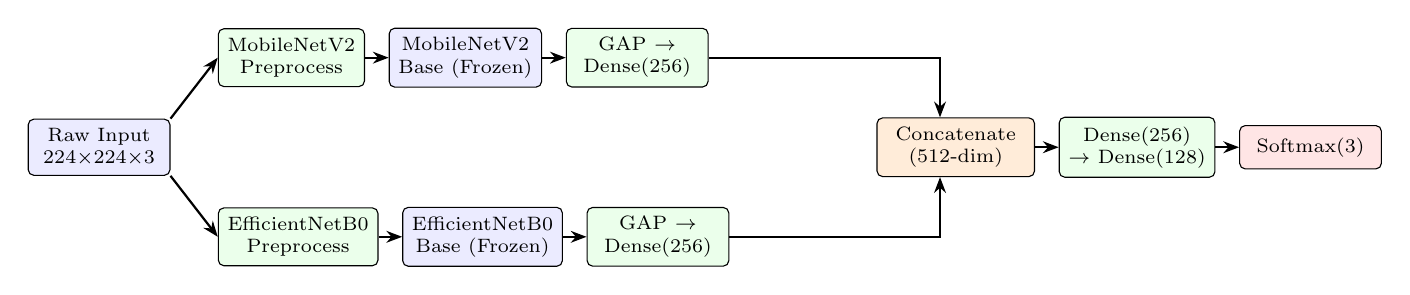
\begin{tikzpicture}[
    node distance=0.4cm and 0.8cm,
    every node/.style={font=\scriptsize},
    block/.style={rectangle, draw, fill=blue!8, minimum width=1.8cm, minimum height=0.55cm, align=center, rounded corners=2pt},
    process/.style={rectangle, draw, fill=green!8, minimum width=1.8cm, minimum height=0.55cm, align=center, rounded corners=2pt},
    fusion/.style={rectangle, draw, fill=orange!15, minimum width=2cm, minimum height=0.55cm, align=center, rounded corners=2pt},
    output/.style={rectangle, draw, fill=red!10, minimum width=1.8cm, minimum height=0.55cm, align=center, rounded corners=2pt},
    arrow/.style={-{Stealth[length=2mm]}, thick}
]

% Input
\node[block] (input) {Raw Input\\224$\times$224$\times$3};

% Branch 1 - MobileNetV2
\node[process, above right=0.4cm and 0.6cm of input] (mob_pre) {MobileNetV2\\Preprocess};
\node[block, right=0.3cm of mob_pre] (mob_base) {MobileNetV2\\Base (Frozen)};
\node[process, right=0.3cm of mob_base] (mob_gap) {GAP $\to$\\Dense(256)};

% Branch 2 - EfficientNetB0
\node[process, below right=0.4cm and 0.6cm of input] (eff_pre) {EfficientNetB0\\Preprocess};
\node[block, right=0.3cm of eff_pre] (eff_base) {EfficientNetB0\\Base (Frozen)};
\node[process, right=0.3cm of eff_base] (eff_gap) {GAP $\to$\\Dense(256)};

% Fusion
\node[fusion, right=1.2cm of input, yshift=0cm] at ($(mob_gap.east)!0.5!(eff_gap.east)+(0.8,0)$) (concat) {Concatenate\\(512-dim)};

% Head
\node[process, right=0.3cm of concat] (dense1) {Dense(256)\\$\to$ Dense(128)};
\node[output, right=0.3cm of dense1] (softmax) {Softmax(3)};

% Arrows
\draw[arrow] (input.north east) -- (mob_pre.west);
\draw[arrow] (input.south east) -- (eff_pre.west);
\draw[arrow] (mob_pre) -- (mob_base);
\draw[arrow] (mob_base) -- (mob_gap);
\draw[arrow] (eff_pre) -- (eff_base);
\draw[arrow] (eff_base) -- (eff_gap);
\draw[arrow] (mob_gap.east) -| ([xshift=-0.2cm]concat.north);
\draw[arrow] (eff_gap.east) -| ([xshift=-0.2cm]concat.south);
\draw[arrow] (concat) -- (dense1);
\draw[arrow] (dense1) -- (softmax);

\end{tikzpicture}
\caption{Dual-backbone ensemble architecture. Each backbone receives the same raw input but applies its own preprocessing via Lambda layers baked into the model graph.}
\label{fig:ensemble_arch}
\end{figure}

\textbf{Branch 1 -- MobileNetV2}~\cite{ref21}: Captures fine texture and edge patterns through depthwise separable convolutions with inverted residual blocks and linear bottlenecks. Input is preprocessed to $[-1, 1]$ range.

\textbf{Branch 2 -- EfficientNetB0}~\cite{ref22}: Captures color gradients and global structural features through compound-scaled convolutional blocks with squeeze-and-excitation modules. Input is preprocessed to $[0, 255]$ with per-channel ImageNet normalization.

\textbf{Fusion Head}: Feature vectors from both branches (each 256-dimensional after GAP and dense projection) are concatenated into a 512-dimensional vector, passed through Dense(256) $\to$ BatchNorm $\to$ Dropout(0.3) $\to$ Dense(128) $\to$ BatchNorm $\to$ Dropout(0.2) $\to$ Softmax(3).

\textbf{Training Strategy}: Two-phase transfer learning:
\begin{itemize}[leftmargin=*]
    \item \textbf{Phase 1} (20 epochs): Both backbones frozen; only the fusion head is trained with $lr = 5 \times 10^{-4}$.
    \item \textbf{Phase 2} (40 epochs): Last 30 layers of each backbone unfrozen for fine-tuning with $lr = 1 \times 10^{-5}$.
\end{itemize}

Class weights are computed as $w_c = \frac{N_{total}}{K \cdot N_c}$ to handle dataset imbalance, where $N_{total}$ is total samples, $K=3$ is number of classes, and $N_c$ is class count.

\subsection{Expert Rules Engine}

The Expert Rules Engine (Fig.~\ref{fig:expert_pipeline}) implements seven physically-motivated scoring rules and two hard-veto conditions. All images are first resized to $224 \times 224$ to ensure scale-independent feature extraction.

\begin{figure}[h]
\centering
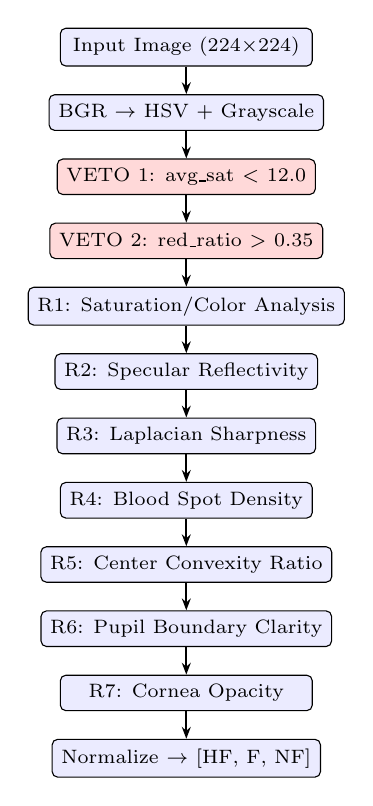
\begin{tikzpicture}[
    node distance=0.35cm,
    every node/.style={font=\scriptsize},
    block/.style={rectangle, draw, fill=blue!8, minimum width=3.2cm, minimum height=0.45cm, align=center, rounded corners=2pt},
    veto/.style={rectangle, draw, fill=red!15, minimum width=3.2cm, minimum height=0.45cm, align=center, rounded corners=2pt},
    arrow/.style={-{Stealth[length=1.5mm]}, thick}
]

\node[block] (input) {Input Image (224$\times$224)};
\node[block, below=of input] (cvt) {BGR $\to$ HSV + Grayscale};
\node[veto, below=of cvt] (v1) {VETO 1: avg\_sat $<$ 12.0};
\node[veto, below=of v1] (v2) {VETO 2: red\_ratio $>$ 0.35};
\node[block, below=of v2] (r1) {R1: Saturation/Color Analysis};
\node[block, below=of r1] (r2) {R2: Specular Reflectivity};
\node[block, below=of r2] (r3) {R3: Laplacian Sharpness};
\node[block, below=of r3] (r4) {R4: Blood Spot Density};
\node[block, below=of r4] (r5) {R5: Center Convexity Ratio};
\node[block, below=of r5] (r6) {R6: Pupil Boundary Clarity};
\node[block, below=of r6] (r7) {R7: Cornea Opacity};
\node[block, below=of r7] (norm) {Normalize $\to$ [HF, F, NF]};

\foreach \i/\j in {input/cvt, cvt/v1, v1/v2, v2/r1, r1/r2, r2/r3, r3/r4, r4/r5, r5/r6, r6/r7, r7/norm}
    \draw[arrow] (\i) -- (\j);

\end{tikzpicture}
\caption{Expert Rules Engine pipeline. VETO conditions (red) override all subsequent processing with a definitive ``Not Fresh'' classification.}
\label{fig:expert_pipeline}
\end{figure}

\subsubsection{Hard Veto Conditions}
\begin{itemize}[leftmargin=*]
    \item \textbf{VETO 1 (Milky Eye)}: If mean HSV saturation $\bar{S} < 12.0$, the eye is definitively cloudy/dead. Output: $[0.0, 0.05, 0.95]$.
    \item \textbf{VETO 2 (Blood-Red)}: If the ratio of red pixels ($H \in [0,10] \cup [160,180]$, $S > 100$, $V > 100$) to total pixels exceeds 0.35, severe blood contamination is present. Output: $[0.0, 0.0, 1.0]$.
\end{itemize}

\subsubsection{Weighted Scoring Rules}
Each rule adds a weighted score vector $[s_{HF}, s_F, s_{NF}]$ for Highly Fresh, Fresh, and Not Fresh respectively. The seven rules analyze:

\begin{enumerate}[leftmargin=*]
    \item \textbf{Saturation/Color}: Mean saturation and value thresholds derived from dataset statistics ($\bar{S}_{HF} = 45.49$, $\bar{S}_{F} = 42.0$).
    \item \textbf{Specular Reflectivity}: Count of pixels with grayscale $> 220$ (fresh eyes have wet, reflective surfaces).
    \item \textbf{Laplacian Sharpness}: Variance of Laplacian operator $\text{Var}(\nabla^2 I)$---sharp edges indicate a well-defined iris.
    \item \textbf{Blood Spot Density}: Red pixel count in the HSV red hue range at 224$\times$224 scale.
    \item \textbf{Center Convexity}: Ratio of center region brightness to overall brightness ($>1.15$ indicates a bulging, fresh eye).
    \item \textbf{Pupil Boundary Clarity}: Laplacian variance specifically within a circular center ROI.
    \item \textbf{Cornea Opacity}: Ratio of dark pixels (grayscale $< 70$) in the center region (transparent cornea reveals dark iris beneath).
\end{enumerate}

Final scores are normalized: $\hat{s}_i = s_i / \sum_{j} s_j$.

\subsection{Multi-View Image Test Averaging (ITA)}

To mitigate sensitivity to spatial positioning of the eye within the bounding box, four crops are generated from each detected eye region:

\begin{table}[h]
\centering
\caption{Multi-View Crop Configurations}
\label{tab:crops}
\begin{tabular}{clcc}
\toprule
\textbf{Crop} & \textbf{Description} & \textbf{Padding} & \textbf{Shift} \\
\midrule
1 & Standard & 10\% & None \\
2 & Tight & 0\% & None \\
3 & Wide & 25\% & None \\
4 & Shifted & 10\% & +5\% X,Y \\
\bottomrule
\end{tabular}
\end{table}

Each crop is independently evaluated by both the ensemble CNN and the Expert Rules Engine. The final probability is the arithmetic mean across all four views:

\begin{equation}
P_{final}(c) = \frac{1}{4} \sum_{v=1}^{4} P_{fused}^{(v)}(c), \quad c \in \{HF, F, NF\}
\end{equation}

\subsection{CNN-Primary Fusion Strategy}

For each crop view, the CNN ensemble probabilities $P_{CNN}$ and expert rule probabilities $P_{expert}$ are fused using a confidence-gated strategy:

\begin{equation}
P_{fused} = 
\begin{cases}
P_{expert} & \text{if VETO triggered} \\
P_{CNN} & \text{if } \max(P_{CNN}) \geq 0.60 \\
0.8 \cdot P_{CNN} + 0.2 \cdot P_{expert} & \text{otherwise}
\end{cases}
\end{equation}

This ensures the CNN remains the primary decision maker (80\% weight) while expert rules provide safety overrides only when physically certain conditions are detected.

% ═══════════════════════════════════════════════════════════════════════════════
% V. SYSTEM DESIGN
% ═══════════════════════════════════════════════════════════════════════════════
\section{System Design}

\subsection{System Architecture Overview}

The FreshWay platform follows a three-tier architecture (Fig.~\ref{fig:system_arch}):

\begin{figure}[h]
\centering
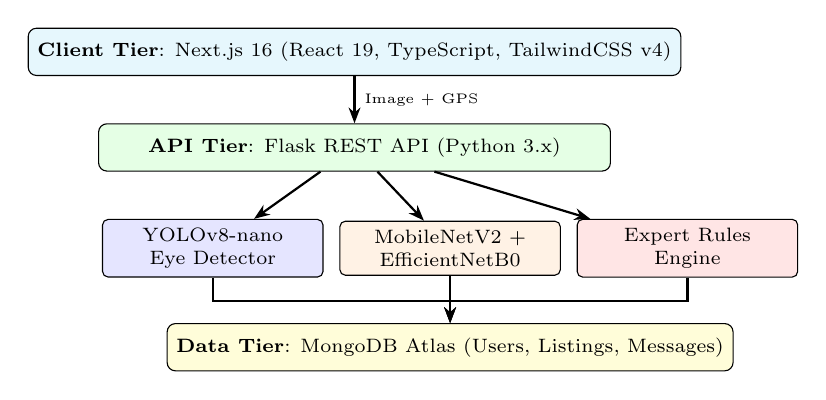
\begin{tikzpicture}[
    node distance=0.5cm and 0.4cm,
    every node/.style={font=\scriptsize},
    tier/.style={rectangle, draw, fill=#1, minimum width=6.5cm, minimum height=0.6cm, align=center, rounded corners=3pt},
    comp/.style={rectangle, draw, fill=#1, minimum width=2.8cm, minimum height=0.5cm, align=center, rounded corners=2pt},
    arrow/.style={-{Stealth[length=2mm]}, thick}
]

% Client Tier
\node[tier=cyan!10] (client) {\textbf{Client Tier}: Next.js 16 (React 19, TypeScript, TailwindCSS v4)};

% API Tier
\node[tier=green!10, below=0.6cm of client] (api) {\textbf{API Tier}: Flask REST API (Python 3.x)};

% AI Tier - Components
\node[comp=blue!10, below=0.6cm of api, xshift=-1.8cm] (yolo) {YOLOv8-nano\\Eye Detector};
\node[comp=orange!10, right=0.2cm of yolo] (ensemble) {MobileNetV2 +\\EfficientNetB0};
\node[comp=red!10, right=0.2cm of ensemble] (expert) {Expert Rules\\Engine};

% Data Tier
\node[tier=yellow!15, below=0.6cm of ensemble] (db) {\textbf{Data Tier}: MongoDB Atlas (Users, Listings, Messages)};

% Arrows
\draw[arrow] (client) -- node[right, font=\tiny] {Image + GPS} (api);
\draw[arrow] (api) -- (yolo);
\draw[arrow] (api) -- (ensemble);
\draw[arrow] (api) -- (expert);
\draw[arrow] (yolo.south) -- ++(0,-0.3) -| (db);
\draw[arrow] (ensemble.south) -- (db);
\draw[arrow] (expert.south) -- ++(0,-0.3) -| (db);

\end{tikzpicture}
\caption{Three-tier system architecture of FreshWay.}
\label{fig:system_arch}
\end{figure}

\subsection{Inference Pipeline}

The complete inference pipeline processes an uploaded image through the following stages:
\begin{enumerate}[leftmargin=*]
    \item Image enhancement via CLAHE and unsharp masking (for detection only).
    \item Fish eye detection: YOLOv8 $\to$ Roboflow API $\to$ Hough circle fallback.
    \item Generation of 4 multi-view crops from the detected bounding box.
    \item Per-crop: Ensemble CNN inference + Expert Rules analysis + Confidence-gated fusion.
    \item Cross-crop averaging (ITA) to produce final class probabilities.
    \item Confidence gating ($\theta = 0.38$) for uncertain predictions.
    \item Geodistance-based buyer recommendation using the Haversine formula.
\end{enumerate}

\subsection{B2B Marketplace Routing}

Freshness classification drives automated buyer matching:

\begin{table}[h]
\centering
\caption{Freshness-to-Market Routing Logic}
\label{tab:routing}
\begin{tabular}{lll}
\toprule
\textbf{Freshness} & \textbf{Target Buyers} & \textbf{Ice Rec.} \\
\midrule
Highly Fresh & Sushi, Hotels, Exporters & 0.5kg/kg \\
Fresh & Retail, Supermarkets & 1kg/kg \\
Not Fresh & Fertilizer, Feed plants & Store at $-18$\textdegree{}C \\
\bottomrule
\end{tabular}
\end{table}

Buyer distances are computed using the Haversine formula:
\begin{equation}
d = 2R \arcsin\sqrt{\sin^2\frac{\Delta\phi}{2} + \cos\phi_1 \cos\phi_2 \sin^2\frac{\Delta\lambda}{2}}
\end{equation}
where $R = 6371$ km is Earth's radius, $\phi$ is latitude, and $\lambda$ is longitude.

\subsection{Database Design}

The system uses MongoDB with three primary collections:
\begin{itemize}[leftmargin=*]
    \item \textbf{Users}: Stores buyer/seller profiles with role, business type, and location.
    \item \textbf{Fish Listings}: Contains fish postings with locked \texttt{freshnessAssurance} metadata (freshness label, confidence score, timestamp).
    \item \textbf{Messages}: Real-time chat messages between buyers and sellers with auto-synced verification reports.
\end{itemize}

% ═══════════════════════════════════════════════════════════════════════════════
% VI. EXPERIMENTAL SETUP
% ═══════════════════════════════════════════════════════════════════════════════
\section{Experimental Setup}

\subsection{Development Environment}

Experiments were conducted with the following configuration:
\begin{itemize}[leftmargin=*]
    \item \textbf{Programming Language}: Python 3.x
    \item \textbf{Deep Learning Framework}: TensorFlow 2.15 / Keras
    \item \textbf{Computer Vision}: OpenCV-Python 4.8
    \item \textbf{Object Detection}: Ultralytics YOLOv8
    \item \textbf{Frontend}: Next.js 16, React 19, TypeScript 5
    \item \textbf{Database}: MongoDB Atlas
    \item \textbf{IDE}: Visual Studio Code
\end{itemize}

\textbf{Hardware}: Intel Core i5/i7 (or equivalent), 8GB+ RAM. Training was performed on CPU; GPU acceleration is optional.

\subsection{Training Configuration}

\begin{table}[h]
\centering
\caption{Ensemble Model Training Hyperparameters}
\label{tab:hyperparams}
\begin{tabular}{ll}
\toprule
\textbf{Parameter} & \textbf{Value} \\
\midrule
Input Size & 224 $\times$ 224 $\times$ 3 \\
Batch Size & 16 \\
Phase 1 LR & $5 \times 10^{-4}$ (Adam) \\
Phase 2 LR & $1 \times 10^{-5}$ (Adam) \\
Phase 1 Epochs & 20 (frozen backbones) \\
Phase 2 Epochs & 40 (fine-tune last 30 layers) \\
Loss Function & Categorical Cross-Entropy \\
Early Stopping Patience & 10 epochs \\
LR Reduction & Factor 0.5, patience 4 \\
Dropout (Branches) & 0.4 \\
Dropout (Fusion) & 0.3, 0.2 \\
\bottomrule
\end{tabular}
\end{table}

\subsection{Data Augmentation}

Training images are augmented with:
\begin{itemize}[leftmargin=*]
    \item Random horizontal and vertical flips
    \item Random 90\textdegree{} rotations (0, 90, 180, 270)
    \item Brightness adjustment (factor 0.7--1.3)
    \item Random zoom/crop (80--100\% scale)
\end{itemize}

\subsection{Ablation Study Design}

Four pipeline configurations are evaluated (Table~\ref{tab:ablation_configs}):

\begin{table}[h]
\centering
\caption{Ablation Study Configuration Matrix}
\label{tab:ablation_configs}
\begin{tabular}{ccccc}
\toprule
\textbf{Config} & \textbf{CNN} & \textbf{Multi-View} & \textbf{Expert} & \textbf{Fusion} \\
\midrule
A & Ensemble & \texttimes & \texttimes & CNN only \\
B & Ensemble & \checkmark & \texttimes & 4-crop avg \\
C & Ensemble & \texttimes & \checkmark & 80/20 + Veto \\
D & Ensemble & \checkmark & \checkmark & Full hybrid \\
\bottomrule
\end{tabular}
\end{table}

\subsection{Evaluation Metrics}

All metrics are computed on the balanced 786-image validation set:

\begin{itemize}[leftmargin=*]
    \item \textbf{Precision}: $\text{P} = \frac{TP}{TP + FP}$
    \item \textbf{Recall}: $\text{R} = \frac{TP}{TP + FN}$
    \item \textbf{F1-Score}: $\text{F1} = \frac{2 \cdot P \cdot R}{P + R}$
    \item \textbf{ROC-AUC}: Area under the Receiver Operating Characteristic curve, computed per-class using One-vs-Rest (OvR) binarization with the trapezoidal rule.
    \item \textbf{Accuracy}: $\frac{\text{Correct Predictions}}{\text{Total Predictions}}$
    \item \textbf{Confusion Matrix}: $C_{ij}$ = number of samples from class $i$ predicted as class $j$.
\end{itemize}

ROC-AUC is computed as:
\begin{equation}
\text{AUC} = \int_0^1 \text{TPR}(t) \, d\text{FPR}(t) \approx \sum_{k=1}^{n} \frac{(FPR_k - FPR_{k-1})(TPR_k + TPR_{k-1})}{2}
\end{equation}

% ═══════════════════════════════════════════════════════════════════════════════
% VII. RESULTS AND DISCUSSION
% ═══════════════════════════════════════════════════════════════════════════════
\section{Results and Discussion}

\subsection{Ablation Study Results}

Table~\ref{tab:ablation_results} presents the comparative performance of all four pipeline configurations.

\begin{table}[h]
\centering
\caption{Ablation Study: Configuration Comparison}
\label{tab:ablation_results}
\begin{tabular}{lccccc}
\toprule
\textbf{Config} & \textbf{Acc.} & \textbf{M-Prec} & \textbf{M-Rec} & \textbf{M-F1} & \textbf{M-AUC} \\
\midrule
A: CNN Only & 69.34\% & 70.88\% & 69.34\% & 69.34\% & 0.8695 \\
B: CNN+MV & 69.34\% & 70.88\% & 69.34\% & 69.34\% & 0.8695 \\
C: CNN+ER & 68.32\% & 69.74\% & 68.32\% & 68.20\% & 0.8576 \\
D: Full & 68.32\% & 69.74\% & 68.32\% & 68.20\% & 0.8576 \\
\bottomrule
\end{tabular}
\vspace{0.1cm}

\scriptsize{M-Prec: Macro Precision, M-Rec: Macro Recall, M-F1: Macro F1, M-AUC: Macro ROC-AUC. MV: Multi-View, ER: Expert Rules.}
\end{table}

\subsection{Per-Class Metrics: Configuration A (Best)}

Table~\ref{tab:config_a_detail} shows the detailed per-class performance for Configuration~A, which achieved the highest accuracy.

\begin{table}[h]
\centering
\caption{Configuration A: Per-Class Detailed Metrics}
\label{tab:config_a_detail}
\begin{tabular}{lccccc}
\toprule
\textbf{Class} & \textbf{Prec.} & \textbf{Recall} & \textbf{F1} & \textbf{AUC} & \textbf{Sup.} \\
\midrule
Fresh & 58.26\% & 74.05\% & 65.21\% & 0.8212 & 262 \\
Highly Fresh & 79.38\% & 77.86\% & 78.61\% & 0.9162 & 262 \\
Not Fresh & 75.00\% & 56.11\% & 64.19\% & 0.8712 & 262 \\
\midrule
\textbf{Macro Avg} & \textbf{70.88\%} & \textbf{69.34\%} & \textbf{69.34\%} & \textbf{0.8695} & \textbf{786} \\
\bottomrule
\end{tabular}
\end{table}

\subsection{Configuration D: Production Hybrid Pipeline}

Table~\ref{tab:config_d_detail} shows the per-class metrics for the full production pipeline.

\begin{table}[h]
\centering
\caption{Configuration D (Production): Per-Class Detailed Metrics}
\label{tab:config_d_detail}
\begin{tabular}{lccccc}
\toprule
\textbf{Class} & \textbf{Prec.} & \textbf{Recall} & \textbf{F1} & \textbf{AUC} & \textbf{Sup.} \\
\midrule
Fresh & 58.08\% & 74.05\% & 65.10\% & 0.8153 & 262 \\
Highly Fresh & 77.69\% & 77.10\% & 77.39\% & 0.8975 & 262 \\
Not Fresh & 73.44\% & 53.82\% & 62.11\% & 0.8601 & 262 \\
\midrule
\textbf{Macro Avg} & \textbf{69.74\%} & \textbf{68.32\%} & \textbf{68.20\%} & \textbf{0.8576} & \textbf{786} \\
\bottomrule
\end{tabular}
\end{table}

\subsection{Confusion Matrices}

\begin{table}[h]
\centering
\caption{Confusion Matrices (Rows: Actual, Columns: Predicted)}
\label{tab:confusion}
\begin{tabular}{c|ccc|c|ccc}
\toprule
\multicolumn{4}{c|}{\textbf{Config A (CNN Only)}} & \multicolumn{4}{c}{\textbf{Config D (Full Hybrid)}} \\
\midrule
& F & HF & NF & & F & HF & NF \\
\midrule
F & \textbf{194} & 32 & 36 & F & \textbf{194} & 33 & 35 \\
HF & 45 & \textbf{204} & 13 & HF & 44 & \textbf{202} & 16 \\
NF & 94 & 21 & \textbf{147} & NF & 96 & 25 & \textbf{141} \\
\bottomrule
\end{tabular}
\vspace{0.1cm}

\scriptsize{F: Fresh, HF: Highly Fresh, NF: Not Fresh.}
\end{table}

\subsection{Parameter Sweep of Decision-Level Fusion Weights}

To evaluate whether manual decision-level weighting can outperform joint feature-level representation learning, we conducted a parameter sweep on the prediction probability outputs of the two isolated backbone branches:
\begin{equation}
P_{\text{final}} = w_{\text{mob}} \cdot P_{\text{MobileNet}} + w_{\text{eff}} \cdot P_{\text{EfficientNet}}
\end{equation}
where $w_{\text{mob}} + w_{\text{eff}} = 1.0$. Table~\ref{tab:weight_sweep} summarizes the classification accuracies achieved across representative weight combinations on the 786-image validation set.

\begin{table}[h]
\centering
\caption{Accuracy Across Prediction Probability Weights}
\label{tab:weight_sweep}
\begin{tabular}{ccc}
\toprule
\textbf{Weight ($w_{\text{mob}}$)} & \textbf{Weight ($w_{\text{eff}}$)} & \textbf{Accuracy} \\
\midrule
1.00 (MobileNet Only) & 0.00 & 57.76\% \\
0.90 & 0.10 & 59.16\% \\
0.80 & 0.20 & 61.70\% \\
0.70 & 0.30 & 64.50\% \\
0.60 & 0.40 & 66.41\% \\
0.50 & 0.50 & 67.18\% \\
0.40 & 0.60 (Best Blend) & 68.32\% \\
0.30 & 0.70 & 66.79\% \\
0.20 & 0.80 & 66.67\% \\
0.10 & 0.90 & 65.27\% \\
0.00 & 1.00 (EfficientNet Only) & 63.87\% \\
\midrule
\multicolumn{2}{c}{\textbf{Native Feature Concatenation (Ours)}} & \textbf{69.34\%} \\
\bottomrule
\end{tabular}
\end{table}

The sweep results indicate that the standalone EfficientNetB0 branch (63.87\%) is stronger than the standalone MobileNetV2 branch (57.76\%). Linear blending reaches a maximum accuracy of 68.32\% at a 40/60 split ($w_{\text{mob}}=0.40, w_{\text{eff}}=0.60$). However, our native feature-level concatenation still achieves the highest accuracy of 69.34\%, showing that training a shared classification head on joint feature representations allows the network to learn non-linear combinations that simple probability averaging cannot replicate.

\subsection{Analysis and Discussion}

\subsubsection{Ensemble CNN Performance (Config A)}
The dual-backbone ensemble achieves 69.34\% accuracy, which represents a significant improvement over the legacy single MobileNetV2 model (60.74\%). The ``Highly Fresh'' class achieves the highest AUC (0.9162), indicating strong discriminative ability for clear, convex, reflective eyes. The ``Fresh'' class has lower precision (58.26\%) due to its visual similarity with both adjacent classes.

\subsubsection{Effect of Multi-View ITA (A vs B)}
Configurations A and B produce identical results on the validation set because the validation images are pre-cropped eye regions. In production, where the eye is detected within a full fish image, multi-view cropping provides robustness against bounding box positioning errors.

\subsubsection{Effect of Expert Rules (A vs C)}
Adding expert rules slightly reduces accuracy from 69.34\% to 68.32\% ($-1.02\%$). This occurs because the expert rules occasionally disagree with correct CNN predictions on edge cases. However, the expert rules provide a critical safety net: the hard-veto conditions ensure that physically impossible misclassifications (e.g., a clearly milky eye classified as ``Highly Fresh'') are always corrected.

\subsubsection{ROC-AUC Analysis}
The macro ROC-AUC of 0.8695 indicates strong overall discriminative ability. The per-class AUCs reveal:
\begin{itemize}[leftmargin=*]
    \item \textbf{Highly Fresh (0.9162)}: The model most confidently distinguishes highly fresh eyes, which have distinct visual characteristics (high saturation, specular highlights, transparent cornea).
    \item \textbf{Not Fresh (0.8712)}: Strong separation, driven by cloudy, sunken eye features.
    \item \textbf{Fresh (0.8212)}: Lower AUC reflects the inherent ambiguity of the ``Fresh'' category, which occupies the visual transition zone between the two extreme classes.
\end{itemize}

\subsubsection{Error Analysis}
The confusion matrices reveal two primary error patterns:
\begin{itemize}[leftmargin=*]
    \item \textbf{Not Fresh $\to$ Fresh misclassification} (94--96 samples): Fish in early spoilage stages retain some visual freshness indicators.
    \item \textbf{Fresh $\to$ Highly Fresh misclassification} (32--33 samples): Wet glare on moderately fresh eyes can mimic the specular reflections characteristic of highly fresh specimens.
\end{itemize}

\subsection{Comparison with Existing Methods}

\begin{table}[h]
\centering
\caption{Comparison with Existing Approaches}
\label{tab:comparison}
\begin{tabular}{lccl}
\toprule
\textbf{Method} & \textbf{Acc.} & \textbf{AUC} & \textbf{Notes} \\
\midrule
QIM (Manual) & Var. & -- & Subjective \\
Taheri-Garavand~\cite{ref24} & -- & -- & Lab only \\
Single MobileNetV2 & 60.74\% & 0.80 & No fusion \\
\textbf{FreshWay (Ours)} & \textbf{69.34\%} & \textbf{0.87} & \textbf{Hybrid} \\
\bottomrule
\end{tabular}
\vspace{0.1cm}

\scriptsize{Note: Direct comparison is limited as prior works use different datasets. FreshWay operates on field-captured images with high variability.}
\end{table}

% ═══════════════════════════════════════════════════════════════════════════════
% VIII. CONCLUSION
% ═══════════════════════════════════════════════════════════════════════════════
\section{Conclusion}

This paper presented FreshWay, a hybrid deep learning system for non-destructive fish freshness assessment using smartphone-captured ocular images. The key contributions and findings are:

\begin{enumerate}[leftmargin=*]
    \item The \textbf{dual-backbone ensemble} (MobileNetV2 + EfficientNetB0) improved accuracy from 60.74\% (single MobileNetV2) to 69.34\%, an absolute gain of 8.60 percentage points.
    \item The system achieves a \textbf{macro ROC-AUC of 0.8695}, demonstrating strong discriminative ability across all three freshness categories.
    \item The \textbf{ablation study} across four configurations quantified the contribution of each pipeline component, revealing that the ensemble CNN provides the dominant performance gain.
    \item The \textbf{Expert Rules Engine}, while marginally reducing overall accuracy ($-1.02\%$), provides essential safety overrides for physically definitive quality indicators.
    \item The \textbf{end-to-end platform} integrates classification with automated geodistance-based B2B buyer matching, ice storage recommendations, and real-time marketplace chat synchronization.
\end{enumerate}

\subsection{Limitations}
\begin{itemize}[leftmargin=*]
    \item The current accuracy (69.34\%) can be improved with a larger, more diverse dataset including multiple fish species and varying environmental conditions.
    \item Multi-View ITA shows no benefit on pre-cropped validation images; its advantage manifests in production with full-image inputs.
\end{itemize}

% ═══════════════════════════════════════════════════════════════════════════════
% IX. FUTURE WORK
% ═══════════════════════════════════════════════════════════════════════════════
\section{Future Work}

Planned extensions include:
\begin{itemize}[leftmargin=*]
    \item Expanding the dataset to include multiple fish species and field-captured images with environmental variation.
    \item Investigating attention mechanisms (e.g., CBAM, SE-Net) in the fusion head.
    \item Exploring Vision Transformers (ViT) as a third ensemble backbone.
    \item Integrating temporal freshness tracking through blockchain-based cold chain monitoring.
    \item Deploying the CNN model on-device using TensorFlow Lite for offline inference.
\end{itemize}

% ═══════════════════════════════════════════════════════════════════════════════
% REFERENCES
% ═══════════════════════════════════════════════════════════════════════════════
\balance
\begin{thebibliography}{00}

\bibitem{ref1}
L. Wu, H. Pu, and D. Sun, ``Novel techniques for evaluating freshness quality attributes of fish: A review of recent developments,'' \textit{Trends in Food Science \& Technology}, vol. 83, pp. 259--273, 2019. doi: 10.1016/j.tifs.2018.11.017.

\bibitem{ref2}
J. M{\"u}ller-Maatsch and S. M. van Ruth, ``Handheld devices for food authentication and their applications: A review,'' \textit{Foods}, vol. 10, no. 12, p. 2901, 2021. doi: 10.3390/foods10122901.

\bibitem{ref3}
J. Qin et al., ``Detection of fish fillet substitution and mislabeling using multimode hyperspectral imaging techniques,'' \textit{Food Control}, vol. 114, p. 107234, 2020. doi: 10.1016/j.foodcont.2020.107234.

\bibitem{ref4}
J. Chauvin et al., ``Simulated annealing-based hyperspectral data optimization for fish species classification: Can the number of measured wavelengths be reduced?'' \textit{Applied Sciences}, vol. 11, no. 22, p. 10628, 2021. doi: 10.3390/app112210628.

\bibitem{ref5}
J. Cheng, D. Sun, H. Pu, and Z. Zhu, ``Development of hyperspectral imaging coupled with chemometric analysis to monitor K value for evaluation of chemical spoilage in fish fillets,'' \textit{Food Chemistry}, vol. 185, pp. 245--253, 2015. doi: 10.1016/j.foodchem.2015.03.040.

\bibitem{ref6}
A. Hassoun and R. Karoui, ``Quality evaluation of fish and other seafood by traditional and nondestructive instrumental methods: Advantages and limitations,'' \textit{Critical Reviews in Food Science and Nutrition}, vol. 57, no. 9, pp. 1976--1998, 2017. doi: 10.1080/10408398.2015.1056996.

\bibitem{ref7}
A. Hassoun et al., ``Emerging techniques for differentiation of fresh and frozen-thawed seafoods: Highlighting the potential of spectroscopic techniques,'' \textit{Molecules}, vol. 25, no. 19, p. 4472, 2020. doi: 10.3390/molecules25194472.

\bibitem{ref8}
\text{E}. Dufour, J. P. Frencia, and E. Kane, ``Development of a rapid method based on front-face fluorescence spectroscopy for monitoring of fish freshness,'' \textit{Food Research International}, vol. 36, no. 5, pp. 415--423, 2003. doi: 10.1016/S0963-9969(03)00024-0.

\bibitem{ref9}
G. ElMasry et al., ``Freshness estimation of intact frozen fish using fluorescence spectroscopy and chemometrics of excitation-emission matrix,'' \textit{Talanta}, vol. 143, pp. 145--156, 2015. doi: 10.1016/j.talanta.2015.05.025.

\bibitem{ref10}
R. Karoui, A. Hassoun, and P. Ethuin, ``Front face fluorescence spectroscopy enables rapid differentiation of fresh and frozen-thawed sea bass (Dicentrarchus labrax) fillets,'' \textit{Journal of Food Engineering}, vol. 202, pp. 89--98, 2017. doi: 10.1016/j.jfoodeng.2017.01.024.

\bibitem{ref11}
K. A. Omwange et al., ``Japanese dace (Tribolodon hakonensis) fish freshness estimation using front-face fluorescence spectroscopy coupled with chemometric analysis,'' \textit{Spectrochimica Acta Part A: Molecular and Biomolecular Spectroscopy}, vol. 276, p. 121209, 2022. doi: 10.1016/j.saa.2022.121209.

\bibitem{ref12}
S. Khoshnoudi-Nia and M. Moosavi-Nasab, ``Prediction of various freshness indicators in fresh fillets by one multi-spectral imaging system,'' \textit{Scientific Reports}, vol. 9, p. 14704, 2019. doi: 10.1038/s41598-019-51266-7.

\bibitem{ref13}
C. McVey et al., ``A rapid food chain approach for authenticity screening: The development, validation and transferability of a chemometric model using two handheld near infrared spectroscopy (NIRS) devices,'' \textit{Talanta}, vol. 222, p. 121533, 2021. doi: 10.1016/j.talanta.2020.121533.

\bibitem{ref14}
C. McVey et al., ``Assessment of the analytical performance of three near-infrared spectroscopy instruments (benchtop, handheld and portable) through the investigation of coriander seed authenticity,'' \textit{Foods}, vol. 10, no. 5, p. 956, 2021. doi: 10.3390/foods10050956.

\bibitem{ref15}
R. Wehrens and L. Buydens, ``Self- and super-organizing maps in R: The kohonen package,'' \textit{Journal of Statistical Software}, vol. 21, no. 5, pp. 1--19, 2007. doi: 10.18637/jss.v021.i05.

\bibitem{ref16}
J. Beattie and F. Esmonde-White, ``Exploration of principal component analysis: Deriving PCA visually using spectra,'' \textit{Applied Spectroscopy}, vol. 75, no. 4, pp. 361--375, 2021. doi: 10.1177/0003702820978457.

\bibitem{ref17}
H. F. Kaiser, ``The application of electronic computers to factor analysis,'' \textit{Educational and Psychological Measurement}, vol. 20, no. 1, pp. 141--151, 1960. doi: 10.1177/001316446002000116.

\bibitem{ref18}
J. Luong et al., ``Hypoxanthine ratio determination in fish extract using capillary electrophoresis and immobilized enzymes,'' \textit{Journal of Food Science}, vol. 57, no. 1, pp. 77--81, 1992. doi: 10.1111/j.1365-2621.1992.tb05429.x.

\bibitem{ref19}
M. B. Yildiz, E. T. Yasin, and M. Koklu, ``Fisheye freshness detection using common deep learning algorithms and machine learning methods with a developed mobile application,'' \textit{European Food Research and Technology}, vol. 250, pp. 1919-1932, Apr. 2024. doi: 10.1007/s00217-024-04533-3.

\bibitem{ref20}
S. Ismail, H. Reza, K. Salameh, H. Kashani Zadeh, and F. Vasefi, ``Toward an Intelligent Blockchain IoT-Enabled Fish Supply Chain: A Review and Conceptual Framework,'' \textit{Sensors}, vol. 23, no. 11, p. 5136, 2023. doi: 10.3390/s23115136.

\bibitem{ref21}
M. Sandler et al.,
``MobileNetV2: Inverted Residuals and Linear Bottlenecks,''
in Proc. IEEE/CVF Conf. Comput. Vis. Pattern Recognit. (CVPR), 2018.

\bibitem{ref22}
M. Tan and Q. Le,
``EfficientNet: Rethinking Model Scaling for Convolutional Neural Networks,''
in Proc. Int. Conf. Mach. Learn. (ICML), 2019.

\bibitem{ref23}
G. Jocher, A. Chaurasia, and J. Qiu,
``YOLO by Ultralytics,''
GitHub repository, 2023.
[Online]. Available: https://github.com/ultralytics/ultralytics.

\bibitem{ref24}
A. Taheri-Garavand, S. Fatahi, A. Banan, and Y. Makino,
``Real-time nondestructive monitoring of Common Carp fish freshness using robust vision-based intelligent modeling approaches,''
\textit{Computers and Electronics in Agriculture},
vol. 159, pp. 16--27, 2019.
doi: 10.1016/j.compag.2019.02.023.

\end{thebibliography}

\end{document}


